%!TEX TS-program = xelatex
\documentclass[12pt]{thesis-umich}

% Swap these lines with the thesis-umich class to enable the memoir build.
% This will have better attention to a proper book layout, but less cons-
% ideration for the Rackham requirements.
%\documentclass[12pt]{memoir}

\usepackage{acronym}
\usepackage{amsmath}
%\usepackage{booktabs}
\usepackage{fontspec}
\usepackage{graphicx}
%\usepackage{listings}
%\usepackage{mathspec}
\usepackage{todonotes}
\usepackage{xcolor}
%\usepackage{xfrac}

\defaultfontfeatures{Mapping=tex-text, Ligatures={Common}}
\setmainfont{TeX Gyre Schola}
\setsansfont{TeX Gyre Heros}
\setmonofont{TeX Gyre Cursor}
%\setmathsfont{TeX Gyre Schola}

\title{Population Kinetics of a Repetitively-Pulsed Nanosecond Discharge}
\author{Benjamin T. Yee}
\department{Nuclear Engineering \& Radiological Sciences}
\year=2013

\frontpagestyle{1}

\dedication{ %
  I would like to dedicate this dissertation to someone else.
}

\acknowledgments[6]{ %
  Who is this?
}
\acknowledgmentswidth{0.8}

\preface[2]{ %
  This is a dissertation about something; I really hope it's good.
}

\committee{ %
  Associate Professor John E. Foster, Chair \\
  Doctor Edward V. Barnat, Sandia National Laboratories \\
  Doctor Isaiah M. Blankson, National Aeronautics and Space Administration \\
  Professor August Evrard \\
  Professor Mark J. Kushner \\
}

\chair{John E. Foster}

\showlistofappendices

\abbreviations{ %
  \acro{rpnd}[\textsc{rpnd}]{repetitively-pulsed nanosecond discharge}
  \acro{dbd}[\textsc{dbd}]{dielectric-barrier discharge}
  \acro{app}[\textsc{app}]{atmospheric-pressure plasma}
  \acro{lte}[\textsc{lte}]{local thermodynamic equilibrium}
}

\begin{document}

  \chapter{Introduction}\label{chp:intro}
    \section{Overview}

Historically, the study of atmospheric-pressure plasmas (\acs{app}'s) is
indistinguishable from the study of plasmas as a whole. However, the detail of
the measurements and calculations associated with \acs{app}'s has been limited
by their complexity. From a computational perspective, the high pressure and
number of potential reactions present a difficult challenge. Likewise, the high
pressure can significantly complicate the data analysis for a number of plasma
diagnostics. Aside from the high pressures, the large electric fields, short
time scales, and general randomness of \acs{app}'s make even the most basic
observations a feat.

In the last several decades, some of this has begun to change. High-powered
computing has allowed simulations with remarkable detail. Similarly, advances in
technology has enabled plasma diagnostics in regimes that were experimentally
inaccessible. As a result, the body of knowledge regarding \acs{app}'s has
greatly increased. Sometimes, the motivation for this work is scientific
curiosity. More often, the study of \acs{app}'s has been driven by a broad range
of applications.

Among the first plasma applications were provided by \acs{app}'s: ozone
generation and lighting. Aside from these items, plasma welding, polymer
treatment, combustion, and plasma televisions have become widely accepted.
Meanwhile, a large number of new applications may soon be added to this list,
including: treatment of tissue wounds, altering airflow over airfoils, and
destruction of industrial pollutants.

Unsurprisingly, each case demands a different kind of plasma. The original arc
discharges were created between two graphite rods connected to immense battery
banks. In contrast, a modern research reactor studying plasma-assisted
combustion might use a fast-switching semiconductor circuit. Over the years,
several types of \acs{app}s have been developed for a variety of situations:
dielectric-barrier, corona, thermal arc, RF, microwave, pulsed, and more.

Within this group\footnote{The interested reader is referred to Starikovskaia's
review \cite{Starikovskaia2006} which provides a general overview of \acs{app}'s
in the context of plasma-assisted combustion}, the repetitively-pulsed
nanosecond discharge (\acs{rpnd}) has created considerable interest. Generally
speaking, a \acs{rpnd} is a plasma generated by a repetitive electrical pulse
applied between two electrodes. The pulse voltage is often in excess of one
kilovolt, lasts anywhere from $<1-100$ ns, and is repeated over a thousand
times each second. The result is a wave of ionization (and light) which crosses
from the powered electrode to the grounded one.

A \acs{rpnd} can fill volumes of several liters with a relatively uniform
plasma. Though they can cause significant excitation of the background gas, they
generally produce very little heating (in some cases below a detection limit of
$\Delta \pm 15$ K). In addition, the excitation can be changed with adjustments
to the magnitude or duration of the electrical pulse. Each of these
characteristics are highly desirable in one or more of potential applications
for \acs{app}'s.

Given all of these promising properties, \acs{rpnd}'s have been the subject of
substantial study by several research groups. However, much of this work has
focused on the physics of \acs{rpnd}'s in air. Unfortunately, air's large number
of constituent elements can lead to notable complexity. In turn, this can
obscure some of the more fundamental questions relation to \acs{rpnd}'s: how do
they form, how is the energy distributed between excited particles, and what
kind of spatial variation can be expected?

This paper details a study of each of these questions in a helium \acs{rpnd}.
Specifically, the densities of one particular excited atom are measured for a
variety of pressures and locations. This is complemented by measurements of the
light emissions for the same set of parameters. A simple model of a \acs{rpnd}
is used to predict several characteristics of the plasma based on the excited
state densities: electron density, electric field, and light emission. The
measured light emissions are interpreted to show how the energy is distributed
in the gas, and how it changes over time. Finally, they are compared with the
estimated light emissions to check the validity of several common assumptions.

\section{Literature Review}

\acs{rpnd}'s are only a recent invention which resulted from advances in
fast-switching semiconductors. However, the physics of their formation is
related to a much larger category of plasmas which includes lightning, sparks,
and even some transient phenomena in DC glows. These plasmas are unique in that
their formation occurs on timescales much faster than the traditional Townsend
mechanism allows for. The means by which these plasmas form has acquired several
names in the literature; here we will adopt the term, fast ionization wave
(\acs{fiw}).\footnote{It should be noted that the phrase wave does not indicate
any kind of periodic motion or spatial arrangement. Simply put, it describes a
boundary which separates ionized and unionized gas which travels from one
electrode to another.}.

\subsection{Early History of Pulsed Discharges}

The first \acs{fiw} was likely generated by Wheatstone in 1835
\cite{Wheatstone1835}. As reported by Thomson \cite{Thomson1893}, Wheatstone
built a vacuum tube six feet in length, and applied a high voltage across the
gas. As a plasma formed in the tube, Wheatstone observed its formation with a
rotating mirror. The use of this apparatus allowed Wheatstone to place a lower
limit on the speed with which the plasma travelled from one electrode to the
other. Though the discharge crossed the tube with a speed of at least
$8\times10^7$ cm/s, spectral observations indicated that the particles emitting
the light were not travelling at that speed \cite{Zahn1879}.

Later, Thomson revisited this work with an improved apparatus
\cite{Thomson1893}. This included a tube that was now 15 m in length and five mm
in diameter, as seen in figure \ref{fig:thomson}.
\begin{figure}
  \centering
  \includegraphics[width=4in]{chapters/introduction/figures/thomson.png}
  \caption{A sketch of J.J. Thomson's early experiments on fast ionization
  waves in long vacuum tubes.}\label{fig:thomson}
\end{figure}
Also using the rotating mirror apparatus, Thomson was able to greatly improve on
the estimates of Wheatstone. He estimated that the so-called ``luminous front''
had a speed that was more than $1.5\times10^{10}$, or in excess of half of the
speed of light. Furthermore, Thomson determined that the front always appeared
to travel from the positively pulsed electrode (anode) to the ground electrode
(cathode).

The study of these luminous fronts was revisited by several researchers in the
wake of Thomson \cite{James1904, Whiddington1925, Beams1926} with varied
success. By his own admission, Beams's work in 1926 was done ``hurriedly,''
using a rudimentary Kerr cell. In 1930, Beams returned to the propagation of
light pulses in vacuum tubes with a rotating mirror apparatus \cite{Beams1930}.
In addition to confirming his previous measurements, and those of Thomson, Beams
discovered that the \acs{fiw} always traveled from the electrode with the
highest absolute potential, to the lowest one. In other words, the wave could be
anode or cathode directed, depending on the magnitude of their potentials
relative to ground. Benefiting from an improved understanding of electricity,
namely the existence of electrons and ions, Beams was able to provide the first
hypothesis on the nature of the \acs{fiw}:
\begin{quote}
  In the neighborhood of the electrode $\ldots{}$ the field is very high and
  intense ionization should take place. This ionization due to the large
  difference in mobilities of positive ions, negative ions and electrons
  respectively should result in the establishment of a space charge. This space
  charge, once formed near the high potential electrode $Q$ must move down the
  tube regardless of the polarity of the applied potential because of the
  changes it produces in the field near its edges.
\end{quote}

At about the same time, Schonland and Collens reported on their observations of
lightning \cite{Schonland1933}. Though the general structure and length scale of
lightning is substantially different from the luminous fronts observed by Beams
and Thomson, the two phenomena would later prove to be very similar. In their
work Schonland and Collens noted that lightning would usually occur in a
two-step process. Based on the images they obtained, they suggested that
the leader was generated by a relatively small ``dart'' with a mean vertical
velocity of $7.2\times10^8$ cm/s. The dart moved in a random manner, changing
directions at random intervals, but always moving downward.

The second step began when this dart reached the ground. Once there, a bright
return stroke would occur along the same path that the leader had traced out. In
contrast to the leader stroke, the return stroke had a velocity of $5\times10^9$
cm/s. Schonland and Collens hesitantly attributed the leader stroke to an
extended electron avalanche, and the return stroke to thermal ionization along
the conductive path generated by the dart. However, calculations by Cravath and
Loeb showed that the speeds of the proposed avalanche would have to be
inconsistent with the fields at the head of a lightning stroke
\cite{Cravath1935}. Instead, they suggested that the dart was actually a moving
region of space charge which locally accelerated electrons to ionizing energies.
This was fundamentally similar to the mechanism proposed by Beams in 1930.

\subsection{The Streamer Model}

It was long known that sparks in air were similar to lightning. Advances in
technology during the 1930's led to experiments which reinforced this
similarity. In response to the measurements of Schonland and Collens; Snoddy,
Beams, and Dietrich studied the breakdown of gas in a long tube with an
oscillograph \cite{Snoddy1936}. The results from the oscillograph showed a very
clear return wave for which they measured several parameters the characterized
as a function of pressure and applied potential. They observed that at low
voltages, the system behaved like a large resistor in series with a capacitor,
and below a critical voltage, no return stroke would form. Finally, in order to
explain the propagation of the \acs{fiw} generated by the positive pulse, they
suggested that photoionization was occurring in the space ahead of the wave.

Around the same time, Flegler and Raether had come to a similar conclusion,
leading to the first attempt at a theory describing streamers
\cite{Flegler1936}. This same theory was proposed independently by Loeb and Meek
in a series of papers \cite{Loeb1940, Loeb1940a, Meek1940}. The streamer theory
divided the initial breakdown of a spark into two steps. In the first step, an
electron avalanche is initiated between two electrodes. The avalanche travels
toward the anode and leaves behind a region of high positive space charge. In
the second step, the return stroke begins at the cathode and travels toward the
cathode. It was suggested that the head of the return stroke ionizes the gas
ahead of it by pulling in background electrons or via photoionization.
\footnote{These early works emphasized the importance of photoionization. It is
now know that it is only required for cathode-directed streamers in systems with
no background ionization. In addition, Mesyats later showed that the lifetime of
the excited states responsible for photoionization were often longer than the
lifetime of the streamers \cite{Mesyats1972}}.

The streamer model proved relatively successful in describing the development of
sparks and lightning. Theoretical estimates of the speed matched the velocity
measurements that were acquired through photographs and oscillographs.
Additionally, the theory is able to account for the halting manner in which
lightning is formed, though it is only tentatively able to describe the
branching and stepped appearance. Finally, the streamer mechanism provides an
adequate explanation of why streamer discharges are not affected by the shape or
material of the cathode, namely, they do not depend on secondary electron
emission.

The study of the formation of streamers and lightning continues to be active to
this day. Following the initial work of Flegler, Raether, Loeb, and Meek, a
number of researchers began to explore the boundary between the Townsend
mechanism and the streamer mechanism. Most notable was Fisher and Bederson's
work in 1951 \cite{Fisher1951}, which was later extended to nitrogen
\cite{Kachickas1952} and argon \cite{Kachickas1953}. However, there were still a
number of phenomena that were poorly explained by the streamer model. In
particular, Kunhardt provided a useful overview of the problems in 1980
\cite{Kunhardt1980}. However, even before that, it was apparent that the
transients of sparks and lightning was more complicated than thought.

\subsection{Ionizing Waves of Potential Gradient}

Per Chalmers \cite{Chalmers1971}, Rogowski and Buss \cite{Rogowski1927,
Buss1932} observed a fast, diffuse, glow discharge immediately prior to the
filaments which often accompany a streamer discharge. Allibone and Meek, noted
similar diffuse discharges in air based on oscillographs and photographs
\cite{Allibone1938, Allibone1938b, Allibone1938c}. However, the Boys apparatus
which was employed in these studies (an ancestor to the modern streak camera)
was unable to capture the evolution of the diffuse glow, given its large spatial
extent.

This was first noted by Allibone who attempted to use Lichtenberg
figures\footnote{Such figures directly exposed photographic emulsions to the
electrical discharge. The developed image was a time-integrated representation
of the discharge.} to definitively capture this diffuse glow
\cite{Allibone1948}. Later, Saxe and Meek used the recently invented
photomultiplier tube to record the evolution of the light emissions in the
brief, diffuse glow \cite{Saxe1948} as a function of space. Both studies
agreed in the existence of the diffuse glow, despite some disagreement on the
nature of its geometry and propagation.

The similarity of fast transient ionization waves in certain glow discharges
\cite{Westberg1959} to those observed in lightning and streamers led Loeb to to
the conclusion that they were all the same phenomena \cite{Loeb1965}. He
referred to them as ``ionizing waves of potential gradient,'' as the proposed
mechanism for the waves was the generation of a steep potential gradient in a
sufficient short period of time. 

As reported by Babich, Loika, and Tarasova \cite{Babich1977}, the detection of
x-ray emissions from pulsed, high-pressure, helium discharges created a new
avenue of interest for these transient plasmas \cite{Stankevich1967,
Noggle1968}. Unlike the streamers, which were often filamentary, these new
discharges exhibited surprising uniformity. The primary difference being the
duration of the pulse (on the order of nanoseconds) and the applied potentials
(in excess of 200 kV).

The x-rays suggested that electrons in these discharges were accelerated to
unusually high energies (on the order of 10 keV) despite the high
collisionality. It was then that Babich and Stankevich suggested that the x-rays
resulted from continually accelerated electrons impinging on the metal
electrodes \cite{Babich1973}. Briefly, the electric fields in the fronts of the
ionizing waves were so large that they managed to accelerate electrons past the
peak in their collisional cross sections.

Mesyats, Bychov, and Kremnev attempted to provide a more rigorous explanation
for the uniform nature of these new discharges \cite{Mesyats1972}. After
conducting several experiments, they came to the conclusion that these transient
plasmas were the result of many overlapping avalanches, unlike the streamer
which only involves a single avalanche. Kunhardt and Byszewski later
expanded on this work by developing a kinetic model to explain the behavior of
all pulsed discharges above the Townsend threshold \cite{Kunhardt1980}.

It was based on the studies of the fast electrons in these discharges that
Mesyats, Bychov, and Kremnev proposed the use of a fast electron beam for
pumping high-pressure gas lasers. Similar work was conducted simultaneously by
Fenstermacher et al.~\cite{Fenstermacher1972}. Palmer \cite{Palmer1974}, and
Levatter and Lin \cite{Levatter1980} determined that there was a threshold
amount of preionization required to ensure homogeneity of the discharge. Hunter
\cite{Hunter1976}, and Koval'chuk and Mesyats \cite{Koval'chuk1976} later
proposed that such discharges be used for fast-closing switches. Gas lasers and
fast switches would drive much of the later research on fast, pulsed discharges.

Eventually these discharges came to be referred to as fast ionization waves
(\acs{fiw}s). A large body of Russian literature developed around their study,
though much of it has remained untranslated. In 1994, Vasilyak produced an
extensive review of these studies \cite{Vasilyak1994}. The data include wave
velocities for a variety of gases and pressures. Other parameters such as
attenuation coefficients for the waves, high energy electron currents, electric
field measurements, and a circuit model of the \acs{fiw} are also included.

\subsection{\textsc{rpnd}s}

Beginning in 1998, the Moscow Institute of Physics and Technology (\acs{mipt})
produced a flurry of studies on the \acs{fiw} \cite{Anikin1998, Pancheshnyi1998,
Starikovskaia1998}. They employed several different diagnostic techniques
(photomultiplier tubes and capacitive probes) in an exceptionally detailed study
in both air and nitrogen, using a shock tube and a bell jar. A summary of these
investigations can be found in \cite{Starikovskaia2001}. The work showed
exceptionally reproducibility of the discharge parameters at relatively low
repetition rates, on the order of tens of Hz, and evidence of runaway electrons.
This work also included some of the first approximations of the electron energy
distribution function (\acs{eedf}).

Interestingly, later analysis of a anode-directed \acs{fiw} in nitrogen by the
group at \acs{mipt} \cite{Pancheshnyi1999} concluded that the, the vast majority
of the electrons were generated \emph{after} the wave. This suggests that the
ionization in an \acs{fiw} does not strictly track the luminous front of the
wave. Additionally, measurements of the conductivity suggested that the local
approximation becomes invalid in the wave front and the electron energy
distribution function resembles a beam.

In 1997 the invention of the fast ionization dynistor (\acs{fid}) was revealed
\cite{Efanov1997}. These new devices enabled sub-nanosecond switching of 10's of
kilovolts, with repetition rates approaching 100 kilohertz. This was a leap
forward over previous technologies which generally used thyristors or spark gaps
for switching. Particularly appealing was the high repetition rate of the
\acs{fid}.

Recall that the volume-filling \acs{fiw} required a significant
amount of preionization. This was often accomplished an ionization source in
addition to the high voltage pulse (in the form of UV radiation, or electron
beams). However, the repetition rates of \acs{fid}s were high enough such that a
substantial number of electrons would carry over between pulses. These seed
electrons obviated the need for a preionization. In addition, the time-averaged
densities of excited states could maintained at much higher values. This had
particular promise for processing applications.

In the eventual commercialization of the \acs{fid} made economically feasible to
create fast, repeatable fast ionization waves. It is this class of discharges
which are now referred to as repetitively-pulsed nanosecond discharges, or
\acs{rpnd}s. Their uniformity, low gas heating, high-pressure operation, and
efficient ionization made them attractive or a number of applications:
\begin{itemize}
  \item plasma-assisted combustion \cite{Starikovskaia2006},
  \item magneto-hydrodynamic energy bypass \cite{Macheret2002},
  \item plasma actuators \cite{Adamovich2009},
  \item and high-pressure xenon lamps \cite{Nikandrov2008, Tsendin2009}.
\end{itemize}

As with the \acs{fiw}s, the primary diagnostics were current and voltage
characteristics, electric field measurements with capacitive probes, and
emission measurements with photomultiplier tubes. Later, intensified \acs{ccd}s
were used to record the emissions of specific transitions as well as broadband
light. This approach has been used to more clearly illustrate the uniformity and
reproducibility of the discharge \cite{Adamovich2009}. Other researchers have
turned to laser-based diagnostics, such as coherent anti-Stokes Raman
scattering, to measure gas heating \cite{Zuzeek2010} and the electric field in
molecular systems \cite{Ito2010, Ito2010a}. Likewise, laser collision-induced
fluorescence (\acs{lcif}) has been used to obtain axial profiles of excited
state and electron densities in helium \acs{rpnd}s \cite{Weatherford2012}.

Concurrent with these improvements in experimental techniques has been similar
progress in the simulation of \textsc{rpnd}s. The one-dimensional models 



  \chapter{Experiment}\label{chp:exp}
    \section{Discharge Apparatus}

The design of the \acs{rpnd} apparatus was similar to the coaxial geometry used
by Vasilyak and others in \acs{fiw} studies \cite{Vasilyak1994}. Broadly, it was
comprised of cylindrical inner conductor, surrounded by a dielectric, surrounded
by an outer conductor. In this case, two electrodes and the \acs{rpnd} between
them served as the inner conductor. The dielectric was provided by a glass tube
and an air gap. Finally, the outer conductor was an aluminum shell. This
configuration has the benefit of minimizing the undesired inductance of the
system which could inhibit the propagation of the exciting voltage pulse.
The geometry and its electrical equivalent are sketched in
figure~\ref{fig:appschem}.
\begin{figure}
  \centering
  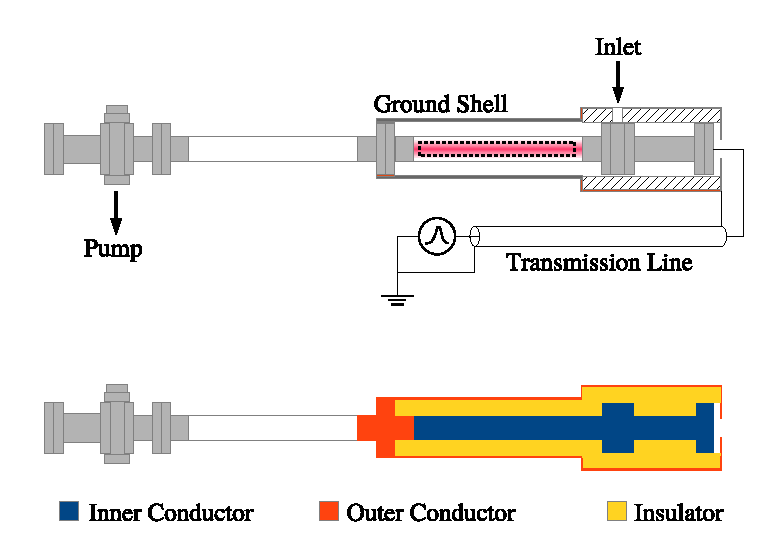
\includegraphics{./chapters/experiment/figures/appschem.eps}
  \caption{Two illustrations of the \acs{rpnd} apparatus. The upper version is
    an annotated sketch of the device, and the bottom version simplifies the
    geometry into its three electrical components.}
  \label{fig:appschem}
\end{figure}
Following from right to left, the inner conductor was composed of a vacuum
window, a Conflat nipple, a double-sided flange tapped for an \textsc{npt}
connection, and the discharge tube containing the plasma.

The tube was composed of borosilicate glass with 2.75 in Conflat flanges on both
ends. The plasma was generated inside the glass tube after it had been evacuated
of air and filled with the desired pressure of helium. The tube had an inner
diameter of 3.3 cm, an outer diameter of 4.0 cm, and a length of 22.9 cm. The
overall length of the tube with the flanges was 30 cm. In the figure shown here,
the right electrode served as the anode, and the left electrode was the cathode.

The dielectric surrounding the inner conductor was composed of several
components. The vacuum window, nipple, double-sided flange, and anode were
separated from the outer conductor by an air gap and a polytetrafluoroethylene
(\acs{ptfe}) tube (hatched in the figure), 20 cm in length with an inner
diameter of about 7.5 cm, and an outer diameter of 10 cm. The plasma portion of
the inner conductor was separated from the outer conductor by an air gap and the
glass tube.

The cathode connected to the outer conductor and served as part of the current
return path. Attached to the cathode was an aluminum tube (referred to as the
ground shell), held in place by a acetyl resin shaft collar and copper
shim.\footnote{While all of the aluminum tube is nominally at ground, it is
likely that it would float to a finite voltage with each pulse.} Radial optical
access to the discharge was provided by two slots milled into the ground shell.
The slots were positioned on opposite sides of the shell and were 3.8 by 25.4 cm
in length. The tube itself was 30 cm in length.

At the end nearest to the anode, the aluminum tube was affixed to a copper
sheet, 10 cm square, with conductive copper tape. A 5 cm diameter hole was cut
into the copper sheet to allow the discharge tube to pass through it. The sheet
was secured to the \acs{ptfe} tube by nylon screws. Surrounding the \acs{ptfe}
tube was a second shell, made of copper sheet. This was connected to the
aluminum tube by a braided copper strap. The right end of the \acs{ptfe} tube
was covered by a second copper sheet, 10 cm square. The sheet was secured to the
\acs{ptfe} tube by nylon screws and in electrical contact with the copper shell.
In the center of the copper sheet was a HN bulkhead adapter for connection to
the transmission line. The inner conductor of the bulkhead adapter was connected
by a straight run of 5 cm of silicone-coated wire to the vacuum window flange.

The voltage pulse was generated by a \acs{fid} power supply, supplied by
\textsc{anvs}, Inc. (model \smaller{PT510NM}). The amplitude of each pulse was
fixed at 6.4 kV with a repetition rate of 1.0 kHz. Each pulse had a fixed width
of 25 ns, with a 10\%-90\% rise time of approximately 4 ns and was roughly
Gaussian in shape. From a practical standpoint, the high impedance prior to
breakdown should effectively double the peak voltage at the anode. A
\textsc{srs} \smaller{DG645} delay generator was used to trigger the power
supply output for all experiments and provided a reference time base for all
measurements.

Preliminary experiments revealed multiple reflections between the power supply
and the anode. A 13.7 m transmission line, made of RG213 coaxial cable, was used
to isolate the reflections so that the effect of individual pulses could be
examined. The calculated delay of the transmission line was 69.2 ns, for a total
separation time between the pulse and the reflection of 138.4 ns. The calculated
delay was found to be a close match in the measured delay.

The gas inlet connection was made through the double-sided flange via a 1/8"
\textsc{npt} hole. A 1/4" polyethylene tube was attached to the \textsc{npt}
connection via a \textsc{npt} to 1/4" Swagelok adapater. The tube was then
connected to a source of ultra-high purity (99.999\%) helium. Throughout the
experiment, the helium flow rate was fixed at 25.0 sccm with a digital flow
controller, regardless of the operating pressure.

The discharge apparatus was pumped down by a oil-based roughing pump with an
upstream zeolite trap. The pump was connected to the discharge tube by a second
glass tube, intended to electrically isolate it from the cathode. The base
pressure of the system was approximately 15 mTorr. The leak rate was measured
several times by evacuating the apparatus and then sealing it from the pump with
a bellows valve. The leak rate was found to be $2.0\times 10^{-3}$ sccm. Given a
constant flow rate of 25.0 sccm, the fractional impurity can be conservatively
estimated to be 80 ppm.

A \textsc{mks} \smaller{PDR-C-2C} power supply and readout, and two capacitance
manometers were used to measure the pressure. One manometer had a full scale
range of 10 Torr, while the other had a range of 100 Torr. The desired pressure
was obtained by sealing the system from the pump with the bellows valve. Two
bypass pump lines, fitted with needle valves, were then used to adjust pumping
speed and system pressure.

The assembled discharge apparatus can be seen in figure~\ref{fig:appphoto}.
\begin{figure}
  \centering
  \setlength\fboxsep{0pt}
  \setlength\fboxrule{1.0pt}
  \fbox{\includegraphics{./chapters/experiment/figures/appphoto.jpg}}
  \caption{Photograph of the discharge apparatus.}
  \label{fig:appphoto}
\end{figure}
The \acs{rpnd} apparatus was supported two 1.5 in mounting posts with angle
brackets. The mounting posts attached to a 4 ft by 2.5 ft optical breadboard,
supported by urethane shock absorbers, and a rigid frame. The roughing pump was
attached to the apparatus with flanged bellows in order to reduce vibrations. 

All electrical measurements were made with a LeCroy \smaller{6100A} WaveRunner
oscilloscope which had a bandwidth of 1.0 GHz. Electrical connections to the
oscilloscope were made with \smaller{RG 50/U} coaxial cable and standard
\textsc{bnc} connectors, terminated at 50 $\Omega$ unless otherwise noted. The
voltage of the pulses was monitored from $1:1000$ divider built into the power
supply. The current was measured from a current shunt located in a break of the
outer conductor of the transmission line. The current shunt was composed of 9,
low inductance, $1.0 \Omega$ resistors connected in parallel.
Figure~\ref{fig:bcs}
\begin{figure}
  \centering
  \setlength\fboxsep{0pt}
  \setlength\fboxrule{1.0pt}
  \fbox{\includegraphics{./chapters/experiment/figures/bcs.jpg}}
  \caption{Photograph of the back-current shunt used to measure the current
  characteristics of the \acs{rpnd}.}
  \label{fig:bcs}
\end{figure}

Data were retrieved from the oscilloscope with a desktop computer via the
\textsc{gpib} interface. Instrument control, data acquisition, and data storage
were all managed by a LabView program. Analog input and output was handled with
the auxiliary input and output ports of a \textsc{srs} \smaller{SR850 DSP}
lock-in amplifier.

\section{Field Calculations}

The electric field characteristics of the discharge system was analyzed using a
two-dimensional, electrostatic solver, Ansoft Maxwell 9. Figure~\ref{fig:fields}
\begin{figure}
  \centering
  \includegraphics{./chapters/experiment/figures/fields.jpg}
  \caption{Heat map and vector plot of the electric field in the \acs{rpnd}
  discharge apparatus.}
  \label{fig:fields}
\end{figure}
is a heat map on a logarithmic scale, of the electric field magnitude, with
overlaid electric field vectors (in magenta). The electric field varies
significantly over the length of the discharge apparatus, with a peak near the
axial location of the glass tube followed by a monotonic decline. These
characteristics are a large departure from simple case of two parallel
electrodes in which the field is uniform throughout. This can be attributed to
the presence of the external ground shield. Though this does complicate the
field characteristics, the proximity of the ground results in a much higher
electric field than would otherwise be achievable.

While the off-axis field lines all feature notable radial components,
particularly close to the anode the center line does not.
Figure~\ref{fig:centere}
\begin{figure}
  \centering
  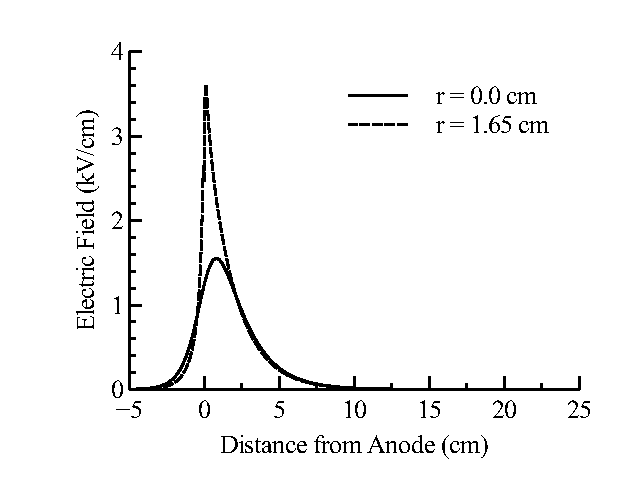
\includegraphics{./chapters/experiment/figures/centere.eps}
  \caption{The magnitude of the electric field along the center and outside of
  the discharge apparatus.}
  \label{fig:centere}
\end{figure}
is a plot of the magnitude of the electric field along the central axis of the
discharge apparatus and the outside, adjacent to the glass tube. The location of
the anode is defined as the location of the glass-to-metal seal. The field close
to the triple point at the seal is the highest at approximately 3.5 kV/cm, while
the field along the axis peaks at about 1.5 kV/cm. At a distance of 2 cm from
the anode, the electric field magnitude is roughly the same regardless of the
radial coordinate. At the measurement locations of 3.83, 11.45, and 19.07 cm,
the vacuum electric field was $4.8 \times 10^5$, 750, and 11 V/m respectively. 

\section{Operating Procedures}

One of two operating procedures was selected depending on how recently the
plasma had last been turned on. If it had been greater than one hour, a full
startup procedure was used. Otherwise, an abbreviated process was used. 

In order to obtain consistent discharge characteristics, it was necessary to
develop two sets of operating procedures for the \acs{rpnd}. In the case that
the discharge had not been operated for over an hour, the roughing pump was
turned on and the primary pump path valve was opened as was the first shutoff
valve upstream of the discharge chamber, seen in figure~\ref{fig:pump}.
\begin{figure}
  \centering
  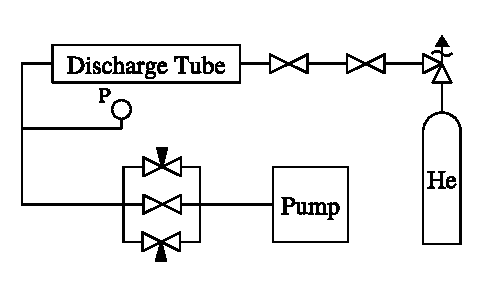
\includegraphics{./chapters/experiment/figures/pump.eps}
  \caption{Simplified diagram of the gas flow path and pumping system.}
  \label{fig:pump}
\end{figure}
The system was then allowed to pump down to its base pressure. Afterward the
final shutoff valve upstream of the pump path was opened and the system was
again allowed to reach base pressure. At this point the helium flow was turned
on and set to 25.0 sccm. The primary pump path was then closed and the needle
valve bypasses were used to adjust the system pressure to 3.0 Torr.

Next, the delay generator was turned on and the output for triggering the power
supply was activated. Then, the \acs{fid} power supply was then turned on. This
would produce an easily visible plasma within the discharge tube. The system was
allowed to operate at this condition for one hour in order to remove potential
contamination on the walls and electrodes. At the end of this period, the pulse
voltage waveform was checked to ensure that it was consistent with previous
waveforms. Once this was confirmed, the pressure was adjusted to the desired
operating condition.

The plasma was shutdown by first shutting off the power supply, followed by the
delay generator. Then, the helium flow was shut off, and the primary pump path
was opened. The system was allowed to come to base pressure before the two
upstream shutoff valves were closed, after which the primary pump path was
closed. The roughing pump was then shut off.

In the cases that the plasma had been operated within the last hour, it was
possible to use an abbreviated startup procedure. This process was fundamentally
the same as the previous one, however the plasma only required five minutes to
reach a steady state. This was verified with multiple measurements of the
current and voltage characteristics as well as the plasma emissions. At times
prior to this five minute equilibration period, the reflected pulse energy was
noticeably higher, and the delay between the trigger pulse and the output pulse
was variable.

\section{Electrical Characteristics}

The general voltage waveform of the \acs{rpnd} showed a number of
characteristics. Figure~\ref{fig:waveform}
\begin{figure}
  \centering
  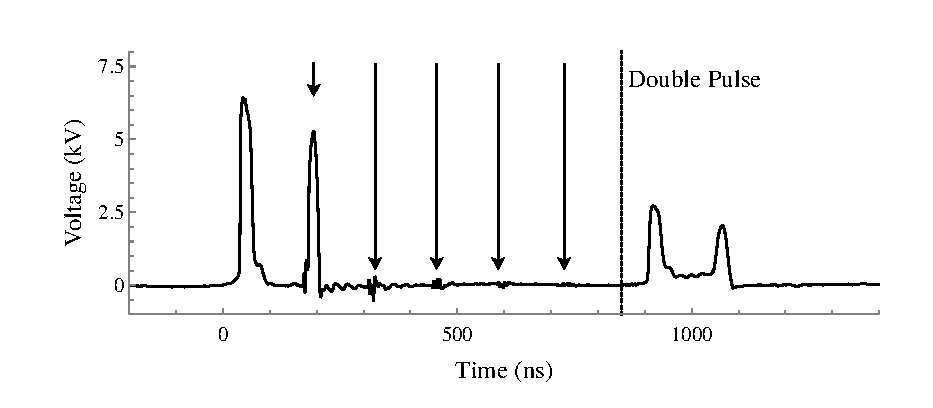
\includegraphics{./chapters/experiment/figures/waveform.eps}
  \caption{Typical voltage waveform of the \acs{rpnd}. Arrows indicate
    reflections back to the power supply. The dotted line delineates the time at
    which the power supply begins to exhibit double pulsing.}
  \label{fig:waveform}
\end{figure}
is a plot of a typical voltage waveform of the \acs{rpnd}. It begins with an
incident pulse with a small foot at $t = 0.0$. This followed by a reflected
pulse 138 ns afterward. The reflected pulse is somewhat attenuated, proportional
to the energy deposited in the plasma. Additional reflections are visible at
integer multiples of 138 ns, however they are highly attenuated. This suggests
that after the first pulse initiates the discharge, energy is much more easily
coupled into the volume. An additional pulse appears after about 800 ns. This is
believed to be a peculiarity of the power supply. For the most part, analysis of
the \acs{rpnd} will focus on the first 138 ns in order to isolate the effects of
a single pulse.

The independent variable for most operating conditions was the pressure of the
system. The properties of the \acs{rpnd} were examined at: 0.3, 0.5, 1.0, 2.0,
3.0, 4.0, 8.0, and 16.0 Torr. The appearance of the plasma varied with the
pressure in a continuous fashion, however it was apparent that there were three
regimes of operation.

At the low pressures, 0.3 and 0.5, it was difficult to initiate the discharge.
Often, it would be necessary to increase the pressure to initiate the discharge,
and then reduce the pressure to the desired conditions. The plasma appeared dim
and relatively constricted to the central axis of the discharge tube, with a
radial extent of approximately 1 cm. Accompanying these presures was a large
degree of electronic noise. This manifested in the voltage and current
waveforms, seen in figure~\ref{fig:waveforms},
\begin{figure}
  \centering
  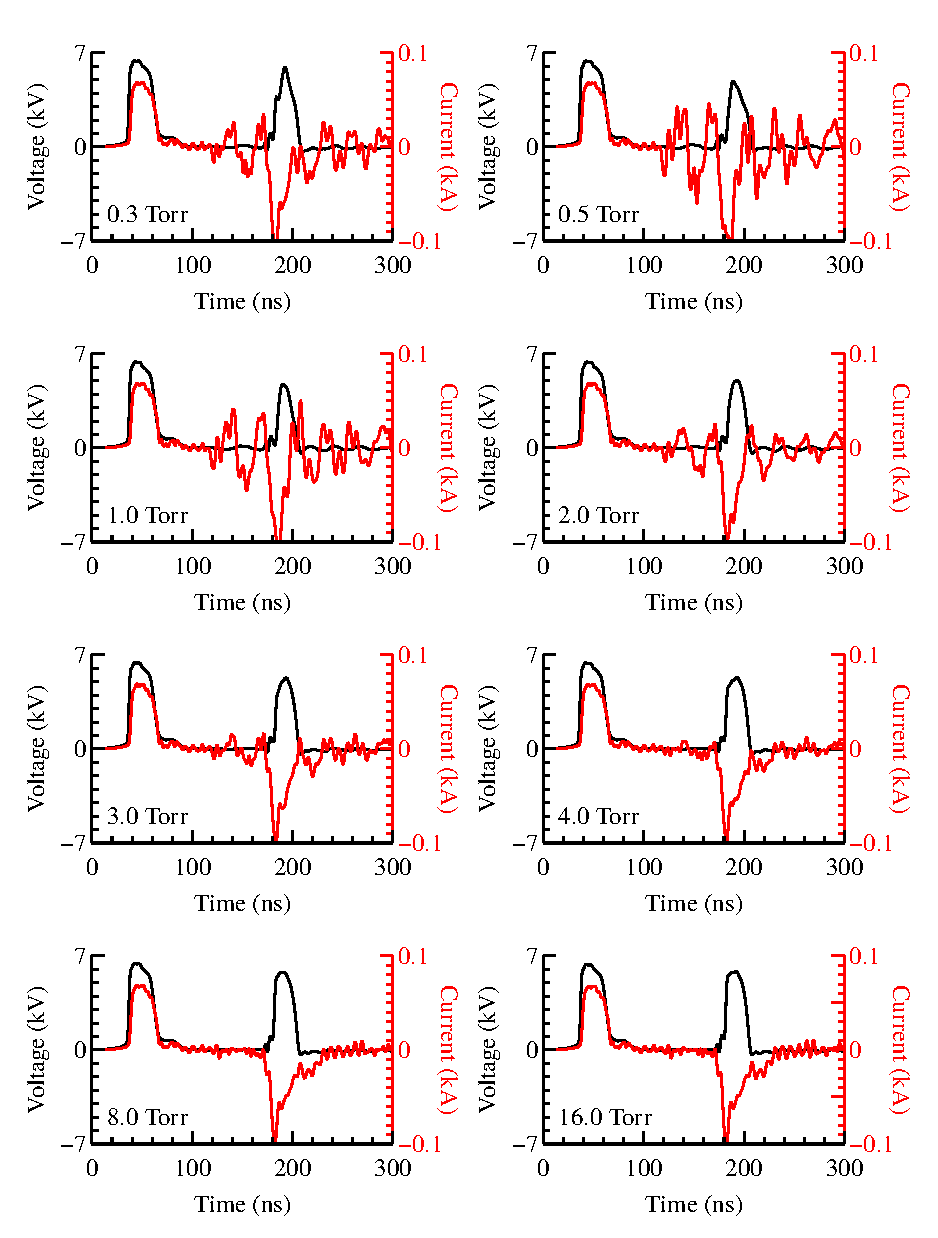
\includegraphics{./chapters/experiment/figures/waveforms.eps}
  \caption{High resolution views of the voltage and current waveforms for the
  first incident and reflected pulse, at each of the operating pressures.}
  \label{fig:waveforms}
\end{figure}
as well as a number of equipment malfunctions.

As the pressure was increased (from 1.0-4.0 Torr), the electrical noise began to
subside. The waveforms in figure~\ref{fig:waveforms} show significant reductions
in the ringing that was particularly prominent in the current waveforms. In
addition, the visual extent of the plasma increased substantially to the point
where it could be considered volume-filling. The plasma also increased its axial
extent as well, eventually reaching well past the cathode/ground. This was
despite attempts to isolate this portion of the apparatus from the plasma. It is
possible to attribute this to the relatively large surface area of the anode in
comparison to the cathode. If a sufficiently high electron current is being
drawn from the cathode, space charge could begin to limit further current
extraction.

However, the plasma receded back to the intended cathode structure at the higher
operating pressures, 8.0 and 16.0 Torr. This was accompanied by a decrease in
the apparent brightness of the plasma to levels similar to that of the low
pressure conditions. In contrast, the plasma appeared to remain volume-filling.
While discharge initiation was difficult at the higher pressures, it was not
accompanied by the electrical noise observed at lower pressures.

\section{Energy Coupling}

The product of the voltage and current waveforms as seen in
figure~\ref{fig:waveforms} gives the power deposited in the plasma as a function
of time. Subsequently, the power integrated over time gives the total energy
deposited in the plasma. However, this approach is somewhat complicated several
features of the \acs{rpnd}. As previously mentioned, the pulses produced by the
power supply are not completely absorbed by the plasma. Therefore, the
integration must be carried out over both the incident and the reflected pulse.
Additionally, there is the concern that the oscillations in the current
measurements could introduce fluctuations in the calculated energy deposition.
However, the small voltage signal limits the error introduced by these
fluctuations to less than 1\%.

Figure~\ref{fig:energies}
\begin{figure}
  \centering
  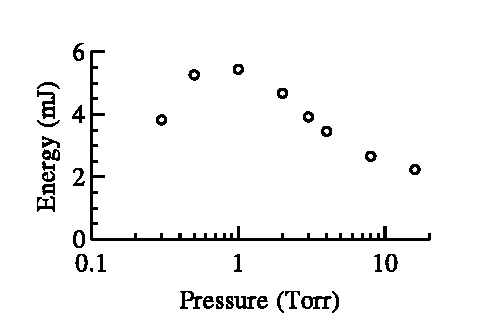
\includegraphics{./chapters/experiment/figures/energies.eps}
  \caption{Plot of the energy coupled into the plasma with the first pulse as
  a function of pressure.}
  \label{fig:energies}
\end{figure}
gives the total energy deposited for the first pulse at each of the operating
conditions. The energy coupled to the plasma peaks at an energy of 5.5 mJ at a
pressure of 1.0 Torr, after which it slowly decreases. This peak in the coupled
energy is coincident with the peak brightness of the plasma. Together, these
suggest that the density of excited states will be optimized at intermediate
pressures. 

Though there appear to be no direct comparisons available in the literature,
several papers report on energy coupling for similar systems. Macheret,
Schneider, and Murray studied a parallel plate \acs{rpnd} in air, at 1-10 Torr
and reported a total energy deposition of 0.30-0.36 mJ, increasing with pressure
\cite{Macheret2006}. Nishihara et al.\ recorded values of 1-2 mJ in a nitrogen
\acs{rpnd} \cite{Nishihara2006}. Pancheshnyi et al., in the study of an
air-propane mixture at 750 Torr, found that each pulse deposited about 1.9 mJ of
energy.

From an applications standpoint, potential existence of a condition which
optimizes the production of excited states is an interesting one. From a
physical standpoint, the growth and decline of energy deposition is with power
is compelling as it suggests two or more competing processes. Though this kind
of competition is reminiscent of Paschen's law, the duration of the pulse is too
short for appreciable ion drift (about 3 mm for the maximum field from the
electrostatic simulations), therefore secondary electron emission is not
important. These observations provide additional impetus for a closer
examination of the \acs{rpnd} properties, particularly the excited states.


  \chapter{Metastable Measurements}\label{chp:meta}
  
  \chapter{Emission Measurements}\label{chp:emit}

  \chapter{Modeling}\label{chp:model}

  \chapter{Conclusions}\label{chp:conc}

  \bibliography{$HOME/Dropbox/References/Thesis}
    \bibliographystyle{unsrt}

\end{document}
